% sage_latex_guidelines.tex V1.20, 14 January 2017
\documentclass[Afour,sagev,times]{sagej}
\usepackage{moreverb,url}

\usepackage[colorlinks,bookmarksopen,bookmarksnumbered,citecolor=red,urlcolor=red]{hyperref}
\usepackage{tikz,makecell,multirow,tablefootnote,threeparttable}
\usetikzlibrary{shapes.geometric, matrix,arrows,positioning,calc,intersections}


\newcommand\BibTeX{{\rmfamily B\kern-.05em \textsc{i\kern-.025em b}\kern-.08em
T\kern-.1667em\lower.7ex\hbox{E}\kern-.125emX}}

\def\volumeyear{2016}

\begin{document}

\runninghead{Smith and Wittkopf}
\title{A technique for constrained optimisation of symmetric laminate using a new
varient of genetic algorithm}
\author{Zhang Huiyao\affilnum{1} and
	Atsushi Yokoyama\affilnum{2*} 
}

\corrauth{Department of Fiber Science and Engineering Kyoto Institute of Techonology, Matsugasaki,
	Sakyo-ku, Kyoto, 606-8585, JAPAN 
}

\email{yokoyama@kit.ac.jp}

\begin{abstract}
The main challenge presented by the design of laminate composite is the laminate layup, involving a
set of fiber orientation, compoiste material system, and stacking sequence. In nature, it is a
combinatorial optimization problem which can be solved by the genetic algorithm(GA). In this present
study, a new varient of GA is introduced to search the optimal design by modifying the selection
strategy. To improve the performance of this new GA, a speical group is maintained in the population
during the optimization process.  To check the feasibility of a laminate subject to in-plane
loading, the effect of fiber orientation angles and materials component on the first ply failure
is studied. A comparative study of basic GA and improved GA in laminate composite designing for
a targeted safety factor is also studied.  An optimal composite material and laminate layup is well
developed for a targeted strength ratio which makes a compromise between weight and cost through
improved genetic algorithm. Numberical results are obtained and presented for different loading
cases.
\end{abstract}

\keywords{Genetic Algorithm, Laminate, Stacking Sequence, Hybrid Composite, Classical Lamination Theory}

\maketitle

\section{1. Introduction}

Composite materials offer improved strength, stiffness, fatigue, and corrosion resistance, etc., over
conventional materials, which are widely used as materials ranging from automotive to ship building
industry, electronic packaging to golf clubs, medical equipment to home building.  However, the high
cost of fabrication of composites is a critical drawback for its application, for example, the
graphite/epoxy composite part may cost as much as \$650 to \$900 per kilogram, while the price of
glass/epoxy is about 2.5 times less. Manufacturing techniques such as sheet molding
compound and structural reinforcement injection molding are taken to lower the cost in manufacturing
automobile parts, and an alternative approach is using of hybrid compoiste material.

The mechanical performance of a laminate compoiste is affected by a wide range of factors,
thickness, material, and orientation of each lamina. Beause of manufacturing limitation, all these
variables are usually limited to a small set of discrete values. For example, ply thickness is fixed 
and ply orientation angles are limited to a set of angles such as 0,45,90 degrees in practice. So the search process for the
optimal design is a discrete optimization problem which can be solved by GA.
To tailor a laminate composite, GA has been successfully
applied to solve laminate design
problem \cite{riche1993optimization,nagendra1996improved,sadagopan1998application,todoroki1998stacking,liu2000permutation,sivakumar1998optimum,walker2003technique,lin2004stacking,kang2005minimum,murugan2007target,akbulut2008optimum}.
GA simulates the process of natural evolutionary includes selection, crossover, 
and mutation according to Darwin's principal of "survival of the fittest".
The known advantage of GA as the following: (i): GAs are not easily trapped in local
optimum, and be able to obtain the global optimum. (ii): GA doesn't need
gradient information and can be applied to discrete optimization problem.
(iii): GA not only be able to find the optimal value in the domain, but also
can maintain a set of optimal solutions. On the other hand, GA also has some disadvantages, 
for example,  the GA needs to evaluate the target functions a lot of times to achieve the
optimization, the cost of the search process is high. The GA consists of some basic parts, the
coding of the design variable, selection strategy, crossover operator, mutation operator, and how to
deal with  constraints.  For the variable design part,  there are two methods to deal with the
representation of design variables, binary string and real value
representation\cite{riche1993optimization,todoroki1998stacking}.
Michalewicz\cite{zbigniew1996genetic} claimed the performance of floating point representation  was
better than binary representation in numerical optimization problem. Selection strategy plays a
critical role in GA which decides the convergence speed and the diversity of the population.  To
improve search ability and reduce search cost, various selection methods have been invented,
and it can be divided into four classes which are proportionate reproduction,
ranking, tournament, and genitor(or ”steady state”) selection. In the optimization of laminate
composite design, roulette wheel\cite{riche1993optimization,seresta2007optimal}, where the
possibility of an individual to be chosen for the next generation is proportional to it's
fitness.  Soremekun \cite{soremekun2001composite} showed that generalized elitist strategy outperformed a
single individual elitism in some special cases.

Data structure, repair strategies and penalty functions\cite{le1995improved} are most common used
approaches to resolve constrained problems in the optimization of composite structure. Symmetric
laminates are widely used in practical scenario, data structure can be used to fulfil the symmetry
constraint which consists of coding a half of the laminate and considering the rest with the
opposite orientation.  Todoroki\cite{todoroki1998stacking} introduced a repair strategy which can
scan the chromosome and repair the gene on the chromosome if it doesn't satisfy the contiguity
constraint. The comparsion of repair strategies in a permutation GA with the same orientation was
presented by Liu\cite{liu2000permutation}, and it showed the Baldwinian repair strategy can
significantly reduce the cost of constrained optimization. Haftka\cite{riche1993optimization} used
GA to solve laminate stacking sequence problem using a penalty function subject to buckling and
strength constraints.


In typical engineering applications, composite materials are under very
complicate loading conditions, not only in-plane loading but also out-of-plane
loading. Most of the studies on the optimization of laminate composite material
was to mimimize the thickness \cite{abu1998optimum,walker2003technique},
weight\cite{fang1993design,deka2005multiobjective,park2008improved}, cost and
weight\cite{deka2005multiobjective,omkar2008artificial}, or maximize the static
strength of composite laminates for a targeted
thickness\cite{walker2003technique,lin2004stacking,kim2007development}. In the
present study, laminate cost and weight are minimized by modifying the objective function.


In order to check the feasibility of a laminate composite by imposing a
strength constraint, failure analysis of a laminate is taken by applying
suitable failure criteria. The failure criteria of laminated composites can be classified in three
classes: non-interactive theories(e.g., Maximum strain), interactive theores(e.g., Tsai-wu), and
parially interactive theories(e.g., Puck failure criterion). The previous researchers adopted the
first-ply-failure approach using the Tsai-wu failure theory
\cite{massard1984computer,reddy1987first,fang1993design,soeiro1994multilevel,pelletier2006multi,jadhav2007parametric,omkar2008artificial,choudhury2019failure},
Tsai-Hill\cite{martin1987optimum,soares1995discrete}, the maximum
stress\cite{jadhav2007parametric,omkar2008artificial}, or the maximum
strain\cite{watkins1987multicriteria} static failure criteria. Akbulut\cite{akbulut2008optimum} used
GA to minimize the thickness of composite laminates with Tsai-Hill and maximum stress failure
criterias, and the advantage of this method is to avoid spurious optima.  Naik\cite{naik2008design}
minimized the weight of laminated composites under restrictions with a failure-mechanism-based
criterion based on Maximum Strian and Tsai-wu.  In the present study, Tsai-wu static failure
criteria is used to investigated the feasibility of a laminate composite.



\section{2. Stress and Strain in a Laminate}
A laminate structure consists of multiple laminas bonded together through
their thickness.  Considering a laminate composite plate which is symmetric to
its middle plane subject to in-plane loading of extension, shear, bending
and torsion,  the classical lamination theory(CLT) is taken to calculate the
stress and strain in the local and global axes of each ply, as shown in
Fig.\ref{fig:lamina}.

\begin{figure*}
	\centering
	\includegraphics[width=\linewidth]{A_laminate_design_images/lamina_local_global_axes.png}
	\caption{Lamina}
  	\label{fig:lamina}
\end{figure*}


\subsection{2.1 Stress and Strian in a Lamina}
For a single lamina, the stress strain relation in the local axis 1-2: 
\begin{equation}
    \begin{bmatrix}
        \sigma_1\\
        \sigma_2\\
        \tau_{12}
    \end{bmatrix}
    =
    \begin{bmatrix}
        Q_{11} & Q_{12} & 0\\
        Q_{12} & Q_{22} & 0\\
        0      &  0     & Q_{66}
    \end{bmatrix}
    \begin{bmatrix}
        \varepsilon_1\\
        \varepsilon_2\\
		\gamma_{12}
    \end{bmatrix}
\end{equation}
Where $Q_{ij}$ are the stiffnesses of the lamina that are related to 
engineering elastic constants given by
\begin{equation}
    \begin{split}
    &Q_{11}=\frac{E_1}{1-v_{12}v_{21}}\\
    &Q_{22}=\frac{E_2}{1-v_{12}v_{21}}\\
    &Q_{66}=G_{12}\\
    &Q_{12}=\frac{v_{21}E_2}{1-v_{12}v_{21}}\\
    \end{split}
\end{equation}

Where, $E_1, E_2, v_{12}, G_{12}$ are four independent engineering elastic constants, they are
defined as 

$E_1$ = longitudinal Young's modulus

$E_2$ = transverse  Young's modulus

$v_{12}$ = major Poisson's ratio

$G_{12}$ = in-plane shear modulus 

Stress strain relation in global axis x-y:  
\begin{equation}
	\left[\begin{array}{l}\sigma_{x} \\ \sigma_{y} \\ \tau_{x
			y}\end{array}\right]=\left[\begin{array}{lll}\bar{Q}_{11} & \bar{Q}_{12} & \bar{Q}_{16}
			\\ \bar{Q}_{12} & \bar{Q}_{22} & \bar{Q}_{26} \\ \bar{Q}_{16} & \bar{Q}_{26} &
			\bar{Q}_{66}\end{array}\right]\left[\begin{array}{l}\varepsilon_{x} \\ \varepsilon_{y}
	\\ \gamma_{x y}\end{array}\right]
\end{equation}

where

\begin{equation}
	\begin{array}{l}
		\bar{Q}_{11}=Q_{11} c^{4}+Q_{22} s^{4}+2\left(Q_{12}+2 Q_{66}\right) s^{2} c^{2}
		\\ 
		\bar{Q}_{12}=\left(Q_{11}+Q_{22}-4 Q_{66}\right) s^{2} c^{2}+Q_{12}\left(c^{4}+s^{2}\right)
		\\ 
		\bar{Q}_{22}=Q_{11} s^{4}+Q_{22} c^{4}+2\left(Q_{12}+2 Q_{66}\right) s^{2} c^{2} \\

		\bar{Q}_{16}=\left(Q_{11}-Q_{12}-2 Q_{66}\right) c^{3} s-\left(Q_{22}-Q_{12}-2
			Q_{66}\right) s^{3} c \\ 
		\bar{Q}_{26}=\left(Q_{11}-Q_{12}-2 Q_{66}\right) c s^{3}-\left(Q_{22}-Q_{12}-2 Q_{66}\right)
		c^{3} s \\ 
		\bar{Q}_{66}=\left(Q_{11}+Q_{22}-2 Q_{12}-2 Q_{66}\right) s^{2}
		c^{2}+Q_{66}\left(s^{4}+c^{4}\right)\\
	\end{array}
\end{equation}
The c and s denotes $cos\theta$, and $sin\theta$. 


The local and global stresses in an angle lamina are related to each other through the angle of
lamina $\theta$
\begin{equation}
	\left[\begin{array}{l}\sigma_{1} \\ \sigma_{2} \\ \tau_{12
			}\end{array}\right]=[T]\left[\begin{array}{l}\sigma_{x} \\ \sigma_{y} \\
	\tau_{xy}\end{array}\right]
\end{equation}

where 

\begin{equation}
	[T]=\left[\begin{array}{ccc}c^{2} & s^{2} & 2 s c \\ s^{2} & c^{2} & -2 s c \\ -s c & s c &
	c^{2}-s^{2}\end{array}\right] 
\end{equation}

\subsection{2.2 Stress and Strain in a Laminate}

\begin{equation} \label{eq:force_and_moments}
	\begin{array}{l}
	\begin{bmatrix}
		N_x \\
		N_y \\
		N_{xy}
	\end{bmatrix}
	=
	\begin{bmatrix}
		A_{11} & A_{12} & A_{16} \\
		A_{12} & A_{22} & A_{26} \\
		A_{16} & A_{26} & A_{66} 
	\end{bmatrix}
    \begin{bmatrix}
		\varepsilon_x^0 \\
        \varepsilon_y^0 \\
		\gamma_{xy}^0
    \end{bmatrix}  
	+ \\ \text{             }
	\begin{bmatrix}
		B_{11} & B_{12} & B_{16} \\
		B_{11} & B_{12} & B_{16} \\
		B_{16} & B_{26} & B_{66} 
	\end{bmatrix}
	\begin{bmatrix}
		k_x \\
		k_y \\
		k_{xy} 
	\end{bmatrix}  \\
	\\

	\begin{bmatrix}
		M_x \\
		M_y \\
		M_{xy}
	\end{bmatrix}
	=
	\begin{bmatrix}
		B_{11} & B_{12} & B_{16} \\
		B_{12} & B_{22} & B_{26} \\
		B_{16} & B_{26} & B_{66} 
	\end{bmatrix}
    \begin{bmatrix}
		\varepsilon_x^0 \\
        \varepsilon_y^0 \\
		\gamma_{xy}^0
    \end{bmatrix} 
	+ \\
	\begin{bmatrix}
		D_{11} & D_{12} & D_{16} \\
		D_{11} & D_{12} & D_{16} \\
		D_{16} & D_{26} & D_{66} 
	\end{bmatrix}
	\begin{bmatrix}
		k_x \\
		k_y \\
		k_{xy} 
	\end{bmatrix}
	\end{array}
\end{equation}

$N_x,N_y$ - normal force per unit length

$N_{xy}$ - shear force per unit length

$M_x,M_y$ - bending moment per unit length

$M_{xy}$ - twisgint moments per unit length

$\varepsilon^0, k$ - mid plane strains, and curvature  of laminate in x-y coordinate

The mid plane strain and curvature is given by

$
\left[\begin{array}{l}\varepsilon^{0} \\ k\end{array}\right]=\left(\begin{array}{ll}A & B \\ B & D\end{array}\right)^{-1}\left\{\begin{array}{l}N \\ M\end{array}\right\}
$






where

\begin{equation}
    \begin{split}
    &A_{ij}
	=
	\sum_{k=1}^n(\overline{Q_{ij}})_k(h_k-h_{k-1})  i=1,2,6, j=1,2,6\\
    &B_{ij}
	=
	\frac{1}{2}\sum_{k=1}^n(\overline{Q_{ij}})_k(h_k-h_{k-1})  i=1,2,6, j=1,2,6\\
    &D_{ij}
	=
	\frac{1}{3}\sum_{k=1}^n(\overline{Q_{ij}})_k(h_k-h_{k-1}) i=1,2,6, j=1,2,6\\
    \end{split}
\end{equation}

The $[A]$, $[B]$, and $[D]$ matrices are called the extensional, coupling, and bending stiffness
matrices. 


\section{3. Failure Theories}
\subsection{3.1 Failure Theories of an Angle Lamina}
Many different theories about the failure of an angle lamina have been developed for a
unidirectional lamina, such as maximum stress failure theory, maximum strain failure theory,
Tsai-Hill failure theory, and Tsai-Wu failure theory. The failure theories of a lamina are based on
the stresses in local axes in the material. There are four normal strength parameters and one shear
stress for a unidirectional lamina. The five strength parameters are

$(\sigma_1^T)_{ult}=$ Ultimate longitudinal tensile strength,

$(\sigma_1^C)_{ult}=$ Ultimate longitudinal compressive strength,

$(\sigma_2^T)_{ult}=$ Ultimate transverse tensile strength,

$(\sigma_2^C)_{ult}=$ Ultimate transverse compressive strength, and

$(\tau_{12})_{ult}=$ Ultimate in-plane shear strength

In the present study, Tsai-wu failure theory is taken to decide whether a lamina is failed or not, the
reason is this theory is  more general than Tsai-Hill failure theory which considers
two different situation, compressive and tensile strength of a lamina. A lamina is considered to be
failed if


\begin{equation} \label{eq:tsai_wu}
\begin{split}
	H_1 \sigma_1 & + H_2 \sigma_2 + H_6 \tau_{12} + H_{11}\sigma_1^2 + H_{22} \sigma_2^2 \\
                 & + H_{66}  \tau_{12}^2 + 2H_{12}\sigma_1\sigma_2 < 1
\end{split}
\end{equation}
 
is violated. where


\begin{equation}
	\begin{array}{l}
		H_{1}=\frac{1}{\left(\sigma_{1}^{T}\right)_{u l t}}-\frac{1}{\left(\sigma_{1}^{C}\right)_{u l
	t}} \\
	H_{11}=\frac{1}{\left(\sigma_{1}^{T}\right)_{u l t}\left(\sigma_{1}^{C}\right)_{u l t}} \\
	H_{2}=\frac{1}{\left(\sigma_{2}^{T}\right)_{u l t}}-\frac{1}{\left(\sigma_{2}^{C}\right)_{u l
	t}} \\
	H_{22}=\frac{1}{\left(\sigma_{2}^{T}\right)_{u l t}\left(\sigma_{2}^{C}\right)_{u l t}} \\
	H_{66}=\frac{1}{\left(\tau_{12}\right)_{u l t}^{2}} \\
	H_{12}=-\frac{1}{2} \sqrt{\frac{1}{\left(\sigma_{1}^{T}\right)_{u l
				t}\left(\sigma_{1}^{C}\right)_{u l t}\left(\sigma_{2}^{T}\right)_{u l
	t}\left(\sigma_{2}^{C}\right)_{u l t}}}
	\end{array}
\end{equation}


The Equation \ref{eq:tsai_wu} can determine whether a lamina failed or not, but it fails to give the
information about how much load can be increased or decreased to keep the lamina safe. The strength
ratio(SR) is to used to solve this problem, and defined as

\begin{equation} \label{eq:sr}
	S R=\frac{\text {Maximum Load Which Can Be Applied}}{\text {Load Applied}}
\end{equation}


Substituting Equation \ref{eq:sr} for $SR$ into Equation \ref{eq:tsai_wu},we obtain
\begin{equation}
	\begin{split}
    	(F_{11}\sigma_1^2 & +F_{22}\sigma_2^2+F_{66}\sigma_6^2+2F_{12}\sigma_1\sigma_2)SR^2 \\ 
						  & +(F_1\sigma_1+F_2\sigma_2)SR-1=0
	 \end{split}
\end{equation}


\subsection{3.2 Failure Theories of a Laminate}
A laminate will fail under increasing mechanical, however, the procedure of laminate failure may not
be catastrophic. In some cases, some layer fail first and the rest is be able to continue to take
more loads until all the plies fail. a ply is fully discount when a ply fails, then the ply is
replaced by near zero stiffness and strength. The procedure for finding the first ply failure in the
present study follows the fully discounted method\cite{daniel1994engineering}:
\begin{enumerate}
	\item Compute the reduced stiffness matrix $[Q]$ referred to local axis for each ply using its
		four engineering elastic constants $E_1$, $E_2$, $v_{12}$, and $G_{12}$.
	\item calculate the transformed reduced stiffness $[\bar{Q}]$ referred to global coordinate
		system (x, y) using reduced stiffness matrix $[Q]$ obtained in step 1 and ply angle for each layer.
	\item Given the thickness $t_k$ and the location of each layer, find out the three laminate
		stiffness matrices $[A]$, $[B]$, and $[D]$.
	\item Apply forces and moments, $[N]_{xy}$, $[M]_{xy}$, solve the equation
		\ref{eq:force_and_moments}, calculate the middle plane strain $[\sigma^0]_{xy}$ and
		cruvature $[k]_{xy}$.
	\item Find out the local strain and stress of each layer under the applied load.
	\item Use the ply-by-ply stresses and strains in Tsai-wu failure theory to find out the strength
		ratio.
\end{enumerate}

\section {4. Optimum Design of Laminate Composite}
\subsection{4.1  Genetic Algorithm}
The GA starts off with a bunch of individuals with limited chromosome length, in which maybe none
of these individuals fulfil the safety factor constraint. The GA is supposed to derive appropriate
offspring based on initial population as the GA goes on. The classic way to handle constrained
search of GA are either introducing repair strategies or using a penaly function, here a new
approach is come up with to deal with constrained GA search problem by modifying the selection
strategy. 

Because of the existence of constraint, it means that the population not only can be sorted by
fitness(which is obtained by objective function), but also can sorted by the constraint value obtained by the constraint function(assuming
constraint function exists), so the
parents of next generation can be chosen by the following two approaches. First, sort out the population by
the absolute difference between the individual's constraint value and the threshold of constraint in an
ascending order, and individual with smaller difference is more likely to be chosen. Individuals
obtained by this method are called potential individuals. Second, sort out the population by
fitness from low to high after remove the unproper individuals, and an individual is proper which
means it fulfils the constraint, and individuals obtained by this way are called proper individuals.
So the final parents consists of two parts, potential individuals and proper individuals, and the
number of potential individuals and proper individual are called, respectively, potential number and
proper number. For example, assumming the parent population is 20, 60 percent of them is
potential individuals, and the rest is proper individuals. So the potential number is 12, and the
proper number is 8.

At the beginning of the GA, no individual in the population is appropriate, which means the
number of proper individuals nearly zero.  So the GA can be divided into two stages according to
whether proper individual are generated during the search process. During the initial stages, the
number of potential individuals gradually decreases from maximum(which is parent population) to the potential
number, while the number of proper individuals increases from zero to the proper number as the GA
goes on. After the initial stage, both of the number of two groups, respectively, converge to
potential number, and proper number.
In order to differentiate the current selection methods from the following, the current GA is called
basic GA. In the following experiment, 50 percent of the parent are potential individuals, and 50
percent of the parent are proper individuals.

The problem with this basic GA is premature and weak local search ability, basic GA are more likely to get stuck in local
optimum. Therefore, to prevent the GA from early convergence and improve the local search
performance, a new selection method is proposed, which is ignoring whether the individual satisfy
the constraint or not, and ranking individuals by their fitness. Individuals selected by
this method are called active individuals, because they are supposed to be always in the population.
GA with this active individuals are called improved GA.
In the improved GA, parents consists of three parts: active individuals, potential 
individuals, and proper individuals. In the following experiment, 20 percent of the parent
population are active individuals, 30 percent of the parent are potential individuals, and the rest
is proper individuals.


In the present study, the relevant parameters of GA are as shown in Table \ref{tab:ga}. The design
variables are the materials, number of layers, and ply orientation restricted to a discrete set of
angles ($0,\pm 45 \text{ and } 90 \text{ degrees} $). The possible materials are graphite/epoxy,
caron/epoxy, and glass/epoxy and are represented by the codes 0, 1 and 2, respectively.

\begin{table*}
\small\sf\centering
\caption{GA parameters}
\begin{tabular}{ccccccc}
	\toprule
	Parameter &  Seed &Population size & LRIC  & Encoding &  Crossover Strategy& Mutation strategy\\
	\midrule
	Value     & 1     &10               & [3-15]& Integer  &  One-point &Mass mutation   \\
	\bottomrule
	\label{tab:ga}
\end{tabular}
\end{table*}
\begin{tablenotes}\footnotesize
\item{"LRIC" denotes the length range of initial chromosome.}
\end{tablenotes}


The laminate chromosome is  represented by a double-gene string
which can be divided into two parts, one part represents the angles, the other
part represents the materials(as shown in Figure \ref{GA:operator}($P_1$)) . To maintain
the diversity of the population, single-point crossover is taken during the
evolution process. The break point in the string are chosen randomly, and one of the offspring of parent 1(as shown in Figure
\ref{GA:operator}($P_1$))  and parent 2(as shown in Figure \ref{GA:operator}($P_2$)) is obtained by combining the
gene segments $P1_o$ and $P2_o$, $P1_m$ and $P2_m$, respectively. The gene code of the offspring
laminate is
$[\text{+}45,\text{-}45,\text{-}45,\text{-}45,\text{-}45,\text{-}45,\text{-}45,0,1,0,1,1,0,1,0]$.

\begin{figure*}
\setlength{\fboxsep}{0pt}%
\setlength{\fboxrule}{0pt}%
\begin{center}
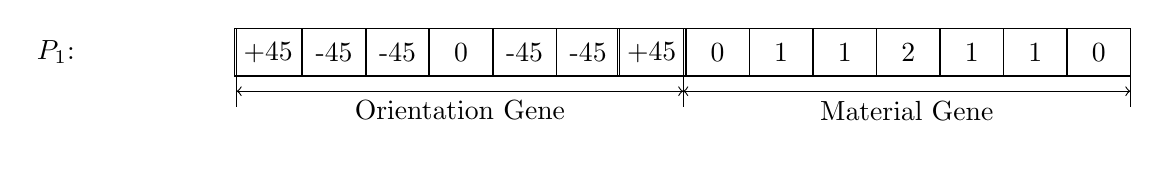
\begin{tikzpicture}
\tikzstyle{rec} = [rectangle, minimum width=0.8cm,minimum height=0.6cm, text
centered, draw=black]
\node (gene11) [rec] {+45};
\node (gene2) [rec] at ($(gene11.east)+(0.4cm,0)$)  {-45};
\node (gene3) [rec] at ($(gene2.east)+(0.4cm,0)$)  {-45};
\node (gene4) [rec] at ($(gene3.east)+(0.4cm,0)$)  {0};
\node (gene5) [rec] at ($(gene4.east)+(0.4cm,0)$)  {-45};
\node (gene6) [rec] at ($(gene5.east)+(0.4cm,0)$)  {-45};
\node (last) [rec] at ($(gene6.east)+(0.4cm,0)$)  {+45};
\node (gene1) [rec] at ($(last.east)+(0.4cm,0)$){0};
\node (gene2) [rec] at ($(gene1.east)+(0.4cm,0)$)  {1};
\node (gene3) [rec] at ($(gene2.east)+(0.4cm,0)$)  {1};
\node (gene4) [rec] at ($(gene3.east)+(0.4cm,0)$)  {2};
\node (gene5) [rec] at ($(gene4.east)+(0.4cm,0)$)  {1};
\node (gene6) [rec] at ($(gene5.east)+(0.4cm,0)$)  {1};
\node (gene7) [rec] at ($(gene6.east)+(0.4cm,0)$)  {0};

\draw[-] ($(gene11.north)+(-0.4cm,0)$) -- ++(0, -1cm) coordinate (A);
\draw[-] ($(last.north)+(0.4cm,0)$) -- ++(0, -1cm) coordinate (B);
\draw[-] ($(gene7.north)+(0.4cm,0)$) -- ++(0, -1cm) coordinate (C);
\draw[<->] ($(A) + (0, 0.2cm)$) -- ($(B) + (0,0.2cm)$) node[pos=0.5,auto=right] {Orientation Gene};
\draw[<->] ($(B) + (0, 0.2cm)$) -- ($(C) + (0,0.2cm)$) node[pos=0.5,auto=right] {Material Gene};
\node[text width=1cm] at ($(gene11.west)+(-2.0cm,0)$) {$P_1$:};
\draw[-] ($(gene11.north)+(0,-1.5cm)$);
\end{tikzpicture}

\begin{tikzpicture}
\tikzstyle{rec} = [rectangle, minimum width=0.8cm,minimum height=0.6cm, text
centered, draw=black]
\node (gene1) [rec] {+45};
\node (gene2) [rec] at ($(gene1.east)+(0.4cm,0)$)  {+45};
\node (gene3) [rec] at ($(gene2.east)+(0.4cm,0)$)  {-45};
\node (gene4) [rec] at ($(gene3.east)+(0.4cm,0)$)  {-45};
\node (gene5) [rec] at ($(gene4.east)+(0.4cm,0)$)  {-45};
\node (gene6) [rec] at ($(gene5.east)+(0.4cm,0)$)  {-45};
\node (gene7) [rec] at ($(gene6.east)+(0.4cm,0)$)  {+45};
\node (last) [rec] at ($(gene7.east)+(0.4cm,0)$)  {+45};
\node (gene1) [rec] at ($(last.east)+(0.4cm,0)$){1};
\node (gene2) [rec] at ($(gene1.east)+(0.4cm,0)$)  {0};
\node (gene3) [rec] at ($(gene2.east)+(0.4cm,0)$)  {0};
\node (gene4) [rec] at ($(gene3.east)+(0.4cm,0)$)  {1};
\node (gene5) [rec] at ($(gene4.east)+(0.4cm,0)$)  {1};
\node (gene6) [rec] at ($(gene5.east)+(0.4cm,0)$)  {0};
\node (gene7) [rec] at ($(gene6.east)+(0.4cm,0)$)  {0};
\node (gene7) [rec] at ($(gene7.east)+(0.4cm,0)$)  {1};

\node[text width=1cm] at ($(gene1.west)+(-6.7cm,0)$) {$P_2$:};
\draw[-] ($(gene11.north)+(0,-1.5cm)$);
\end{tikzpicture}

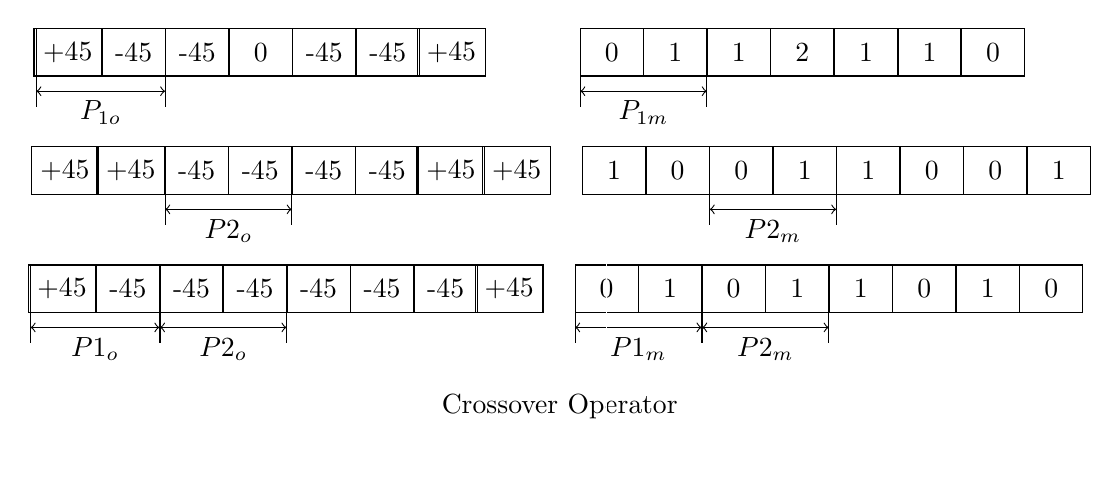
\begin{tikzpicture}
\tikzstyle{rec} = [rectangle, minimum width=0.8cm,minimum height=0.6cm, text
centered, draw=black]
\node (gene11) [rec] {+45};
\node (gene2) [rec] at ($(gene11.east)+(0.4cm,0)$)  {-45};
\node (gene3) [rec] at ($(gene2.east)+(0.4cm,0)$)  {-45};
\node (gene4) [rec] at ($(gene3.east)+(0.4cm,0)$)  {0};
\node (gene5) [rec] at ($(gene4.east)+(0.4cm,0)$)  {-45};
\node (gene6) [rec] at ($(gene5.east)+(0.4cm,0)$)  {-45};
\node (last) [rec] at ($(gene6.east)+(0.4cm,0)$)  {+45};

\draw[-] ($(gene11.north)+(-0.4cm,0)$) -- ++(0, -1cm) coordinate (A);
\draw[-] ($(gene2.north)+(0.4cm,0)$) -- ++(0, -1cm) coordinate (B);
\draw[<->] ($(A) + (0, 0.2cm)$) -- ($(B) + (0,0.2cm)$) node[pos=0.5,auto=right] {$P_{1o}$};
\node (gene1) [rec] at ($(last.east)+(1.6cm,0)$){0};
\node (gene2) [rec] at ($(gene1.east)+(0.4cm,0)$)  {1};
\node (gene3) [rec] at ($(gene2.east)+(0.4cm,0)$)  {1};
\node (gene4) [rec] at ($(gene3.east)+(0.4cm,0)$)  {2};
\node (gene5) [rec] at ($(gene4.east)+(0.4cm,0)$)  {1};
\node (gene6) [rec] at ($(gene5.east)+(0.4cm,0)$)  {1};
\node (gene7) [rec] at ($(gene6.east)+(0.4cm,0)$)  {0};
\draw[-] ($(gene1.north)+(-0.4cm,0)$) -- ++(0, -1cm) coordinate (A);
\draw[-] ($(gene2.north)+(0.4cm,0)$) -- ++(0, -1cm) coordinate (B);
\draw[<->] ($(A) + (0, 0.2cm)$) -- ($(B) + (0,0.2cm)$) node[pos=0.5,auto=right] {$P_{1m}$};

% parent2 

\node (genep2) [rec] at ($(gene11.west)+(0.4cm,-1.5cm)$) {+45};
\node (gene2) [rec] at ($(genep2.east)+(0.4cm,0)$)  {+45};
\node (gene3) [rec] at ($(gene2.east)+(0.4cm,0)$)  {-45};
\node (gene4) [rec] at ($(gene3.east)+(0.4cm,0)$)  {-45};
\node (gene5) [rec] at ($(gene4.east)+(0.4cm,0)$)  {-45};
\node (gene6) [rec] at ($(gene5.east)+(0.4cm,0)$)  {-45};
\node (gene7) [rec] at ($(gene6.east)+(0.4cm,0)$)  {+45};
\node (last) [rec] at ($(gene7.east)+(0.4cm,0)$)  {+45};
\draw[-] ($(gene3.north)+(-0.4cm,0)$) -- ++(0, -1cm) coordinate (A);
\draw[-] ($(gene4.north)+(0.4cm,0)$) -- ++(0, -1cm) coordinate (B);
\draw[<->] ($(A) + (0, 0.2cm)$) -- ($(B) + (0,0.2cm)$) node[pos=0.5,auto=right] {$P2_o$};
\node (gene1) [rec] at ($(last.east)+(0.8cm,0)$){1};
\node (gene2) [rec] at ($(gene1.east)+(0.4cm,0)$)  {0};
\node (gene3) [rec] at ($(gene2.east)+(0.4cm,0)$)  {0};
\node (gene4) [rec] at ($(gene3.east)+(0.4cm,0)$)  {1};
\node (gene5) [rec] at ($(gene4.east)+(0.4cm,0)$)  {1};
\node (gene6) [rec] at ($(gene5.east)+(0.4cm,0)$)  {0};
\node (gene7) [rec] at ($(gene6.east)+(0.4cm,0)$)  {0};
\node (gene7) [rec] at ($(gene7.east)+(0.4cm,0)$)  {1};
\draw[-] ($(gene3.north)+(-0.4cm,0)$) -- ++(0, -1cm) coordinate (A);
\draw[-] ($(gene4.north)+(0.4cm,0)$) -- ++(0, -1cm) coordinate (B);
\draw[<->] ($(A) + (0, 0.2cm)$) -- ($(B) + (0,0.2cm)$) node[pos=0.5,auto=right] {$P2_m$};

% offspring

\node (gene1) [rec] at ($(genep2.west)+(0.4cm,-1.5cm)$) {+45};
\node (gene2) [rec] at ($(gene1.east)+(0.4cm,0)$)  {-45};
\node (gene3) [rec] at ($(gene2.east)+(0.4cm,0)$)  {-45};
\node (gene4) [rec] at ($(gene3.east)+(0.4cm,0)$)  {-45};
\node (gene5) [rec] at ($(gene4.east)+(0.4cm,0)$)  {-45};
\node (gene6) [rec] at ($(gene5.east)+(0.4cm,0)$)  {-45};
\node (gene7) [rec] at ($(gene6.east)+(0.4cm,0)$)  {-45};
\node (last) [rec] at ($(gene7.east)+(0.4cm,0)$)  {+45};

\draw[-] ($(gene1.north)+(-0.4cm,0)$) -- ++(0, -1cm) coordinate (A);
\draw[-] ($(gene2.north)+(0.4cm,0)$) -- ++(0, -1cm) coordinate (B);
\draw[<->] ($(A) + (0, 0.2cm)$) -- ($(B) + (0,0.2cm)$) node[pos=0.5,auto=right] {$P1_o$};

\draw[-] ($(gene3.north)+(-0.4cm,0)$) -- ++(0, -1cm) coordinate (A);
\draw[-] ($(gene4.north)+(0.4cm,0)$) -- ++(0, -1cm) coordinate (B);
\draw[<->] ($(A) + (0, 0.2cm)$) -- ($(B) + (0,0.2cm)$) node[pos=0.5,auto=right] {$P2_o$};

\node (gene1) [rec] at ($(last.east)+(0.8cm,0)$){0};
\node (gene2) [rec] at ($(gene1.east)+(0.4cm,0)$)  {1};
\node (gene3) [rec] at ($(gene2.east)+(0.4cm,0)$)  {0};
\node (gene4) [rec] at ($(gene3.east)+(0.4cm,0)$)  {1};
\node (gene5) [rec] at ($(gene4.east)+(0.4cm,0)$)  {1};
\node (gene6) [rec] at ($(gene5.east)+(0.4cm,0)$)  {0};
\node (gene7) [rec] at ($(gene6.east)+(0.4cm,0)$)  {1};
\node (gene7) [rec] at ($(gene7.east)+(0.4cm,0)$)  {0};

\draw[-] ($(gene1.north)+(-0.4cm,0)$) -- ++(0, -1cm) coordinate (A);
\draw[-] ($(gene2.north)+(0.4cm,0)$) -- ++(0, -1cm) coordinate (B);
\draw[<->] ($(A) + (0, 0.2cm)$) -- ($(B) + (0,0.2cm)$) node[pos=0.5,auto=right] {$P1_m$};
\draw[-] ($(gene3.north)+(-0.4cm,0)$) -- ++(0, -1cm) coordinate (A);
\draw[-] ($(gene4.north)+(0.4cm,0)$) -- ++(0, -1cm) coordinate (B);
\draw[<->] ($(A) + (0, 0.2cm)$) -- ($(B) + (0,0.2cm)$) node[pos=0.5,auto=right] {$P2_m$};

\node[text width=3cm] at ($(gene1.east)+(-1.0cm,-1.5cm)$)  {Crossover Operator};
\draw[-,white] ($(gene1.north)$)-- ++(0,-2.5cm);
\end{tikzpicture}

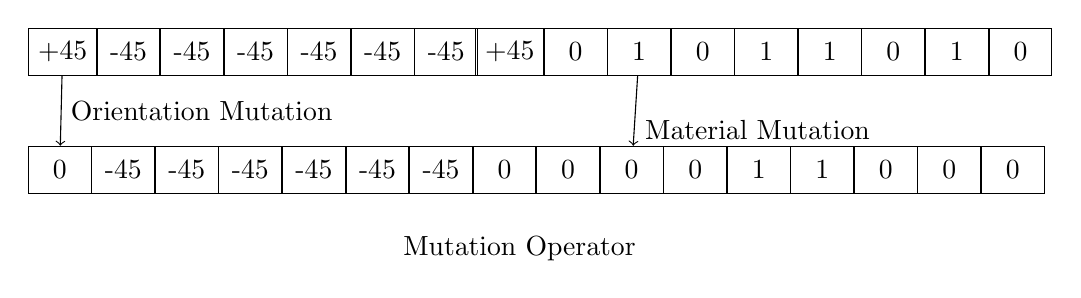
\begin{tikzpicture}
\tikzstyle{rec} = [rectangle, minimum width=0.8cm,minimum height=0.6cm, text
centered, draw=black]
\node (gene11) [rec] {+45};
\node (gene2) [rec] at ($(gene11.east)+(0.4cm,0)$)  {-45};
\node (gene3) [rec] at ($(gene2.east)+(0.4cm,0)$)  {-45};
\node (gene4) [rec] at ($(gene3.east)+(0.4cm,0)$)  {-45};
\node (gene5) [rec] at ($(gene4.east)+(0.4cm,0)$)  {-45};
\node (gene6) [rec] at ($(gene5.east)+(0.4cm,0)$)  {-45};
\node (gene7) [rec] at ($(gene6.east)+(0.4cm,0)$)  {-45};
\node (last) [rec] at ($(gene7.east)+(0.4cm,0)$)  {+45};
\node (gene1) [rec] at ($(last.east)+(0.4cm,0)$){0};
\node (gene2u) [rec] at ($(gene1.east)+(0.4cm,0)$)  {1};
\node (gene3) [rec] at ($(gene2u.east)+(0.4cm,0)$)  {0};
\node (gene4) [rec] at ($(gene3.east)+(0.4cm,0)$)  {1};
\node (gene5) [rec] at ($(gene4.east)+(0.4cm,0)$)  {1};
\node (gene6) [rec] at ($(gene5.east)+(0.4cm,0)$)  {0};
\node (gene7) [rec] at ($(gene6.east)+(0.4cm,0)$)  {1};
\node (gene7) [rec] at ($(gene7.east)+(0.4cm,0)$)  {0};

\node (gene12) [rec] at ($(gene11.west)+(0.4cm,-1.5cm)$) {0};
\node (gene2) [rec] at ($(gene12.east)+(0.4cm,0)$)  {-45};
\node (gene3) [rec] at ($(gene2.east)+(0.4cm,0)$)  {-45};
\node (gene4) [rec] at ($(gene3.east)+(0.4cm,0)$)  {-45};
\node (gene5) [rec] at ($(gene4.east)+(0.4cm,0)$)  {-45};
\node (gene6) [rec] at ($(gene5.east)+(0.4cm,0)$)  {-45};
\node (gene7) [rec] at ($(gene6.east)+(0.4cm,0)$)  {-45};
\node (last) [rec] at ($(gene7.east)+(0.4cm,0)$)  {0};
\node (gene1) [rec] at ($(last.east)+(0.4cm,0)$)  {0};
\node (gene2d) [rec] at ($(gene1.east)+(0.4cm,0)$)  {0};
\node (gene3) [rec] at ($(gene2d.east)+(0.4cm,0)$)  {0};
\node (gene4) [rec] at ($(gene3.east)+(0.4cm,0)$)  {1};
\node (gene5) [rec] at ($(gene4.east)+(0.4cm,0)$)  {1};
\node (gene6) [rec] at ($(gene5.east)+(0.4cm,0)$)  {0};
\node (gene7) [rec] at ($(gene6.east)+(0.4cm,0)$)  {0};
\node (gene7) [rec] at ($(gene7.east)+(0.4cm,0)$)  {0};

\draw[->] (gene11) -- (gene12) node[pos=0.5,auto=left] {Orientation Mutation};
\draw[->] (gene2u) -- (gene2d) node[pos=0.5,auto=left] {Material Mutation};
\node[text width=3cm] at ($(gene1.east)+(-1.0cm,-1cm)$)  {Mutation Operator};
\end{tikzpicture}
\end{center}
\caption{GA Operators\label{GA:operator}}
\end{figure*}

To prevent the
search from getting stuck in a local optimum, mutation is used to random change
the gene in the chromosome, the offspring after mutation operator is as shown
in Figure \ref{GA:operator}

The GA is a stochastic procedure which heavily depends on the generator of pseudo random numbers. In
the present study, the standard Wichmann-Hill generator is used in the algorithm, which combines
three pure multiplicative congruential generators of modulus 30269, 30307 and 30323.  The seed used
in this paper is 1.


\subsection{4.2 Design Problem I}

The aim is to minimize the mass of a laminate composite for a targeted strength
ratio by Tsai-wu failure theory. The design variable are the ply angles, and the
number of layers.

Find: $\{\theta_k, n\}$ $\theta_k \in \{ 0,\text{+}45,\text{-}45,90\}$ 

Minimize: weight

Subject to: strength ratio and first ply failure constraint


\subsection{4.3 Design Problem II}
The aim is to mimimize the weighted cost and weight of hybrid composite
laminate under various loading cases, so the design variable not only include
the ply angles and number of layers, but also the material of each lamina. 


Find: $\{\theta_k,\text{mat}_k, n\}$ $\theta_k \in \{ 0,\text{+}45,\text{-}45,90\}$ $\text{mat}_k \in \{CA, GR, GL \}$

Minimize: 
\begin{equation}
	F=\frac{\text { Cost }}{C_{\text {min }}}+\frac{\text { Weight }}{W_{\text {min }}}
\end{equation}

Subject to: strength ratio and first ply failure constraint


Here CA, GF, and GL represent carbon/epoxy, graphite/epoxy, and glass/epoxy,
 $C_{\text{min}}$ and $W_{\text{min}}$ represent the cost and
weight corresponding to the laminates with minimum cost and minimum weight
obtained from previous problem.

\section{5. Numberical Results and Discussion}
A laminate composite with dimensions $1000 \times 1000 \times 0.165 mm^3$ of
each lamina is under various loading cases, and each CA, GF, and GL layer is
assumed to cost 8, 2.5 and 1 monetary units, respectively.  The other used
material properties are as shown in Table \ref{tab:mat}.  In the present
experiment,  the optimal composite system, layup, thickness, and number of
layers for a targeted strength ratio(2 in this paper) under two different
in-plane loading is investigated.

The programming language Python3 is employed to implement the genetic algorithm, which is a
high-level object-oriented language, and it's grammar is very concise and easy to pick up.


\begin{table*}
\small\sf\centering
\caption{Comparsion of carbon/epoxy, graphite/epoxy, and glass/epoxy properties}
\begin{tabular}{cccccc}
	\toprule
	Property								   & Symbol				  & Unit  &  Carbon/Epoxy&  Graphite/Epoxy  &  Glass/Epoxy   \\
	\midrule																								  
	Longitudinal elastic modulus			   & $E_1$				  & GPa   &  116.6       &  181             &  38.6           \\
	Traverse elastic modulus				   & $E_2$				  & GPa   &  7.67        &  10.3            &  8.27           \\
	Major Poisson's ratio					   & $v_{12}$			  &       &  0.27        &  0.28            &  0.26           \\
	Shear modulus							   & $G_{12}$			  & GPa   &  4.17        &  7.17            &  4.14           \\
	Ultimate longitudinal tensile strength     & $(\sigma_1^T)_{ult}$ & MP    &  2062        &  1500            &  1062            \\
	Ultimate longitudinal compressive strength & $(\sigma_1^C)_{ult}$ & MP    &  1701        &  1500            &  610             \\
	Ultimate transverse tensile strength       & $(\sigma_2^T)_{ult}$ & MPa   &  70          &  40              &  31              \\
	Ultimate transverse compressive strength   & $(\sigma_2^C)_{ult}$ & MPa   &  240         &  246             &  118              \\
	Ultimate in-plane shear strength           & $(\tau_{12})_{ult}$  & MPa   &  105         &  68              &  72               \\
	Density                                    & $\rho$               & $g/cm^3$ &  1.605    &  1.590           &  1.903               \\
	Cost                                       &                      &       &  8           &  2.5             &  1               \\
	\bottomrule
\end{tabular}
\label{tab:mat}
\end{table*}

\begin{figure*}
  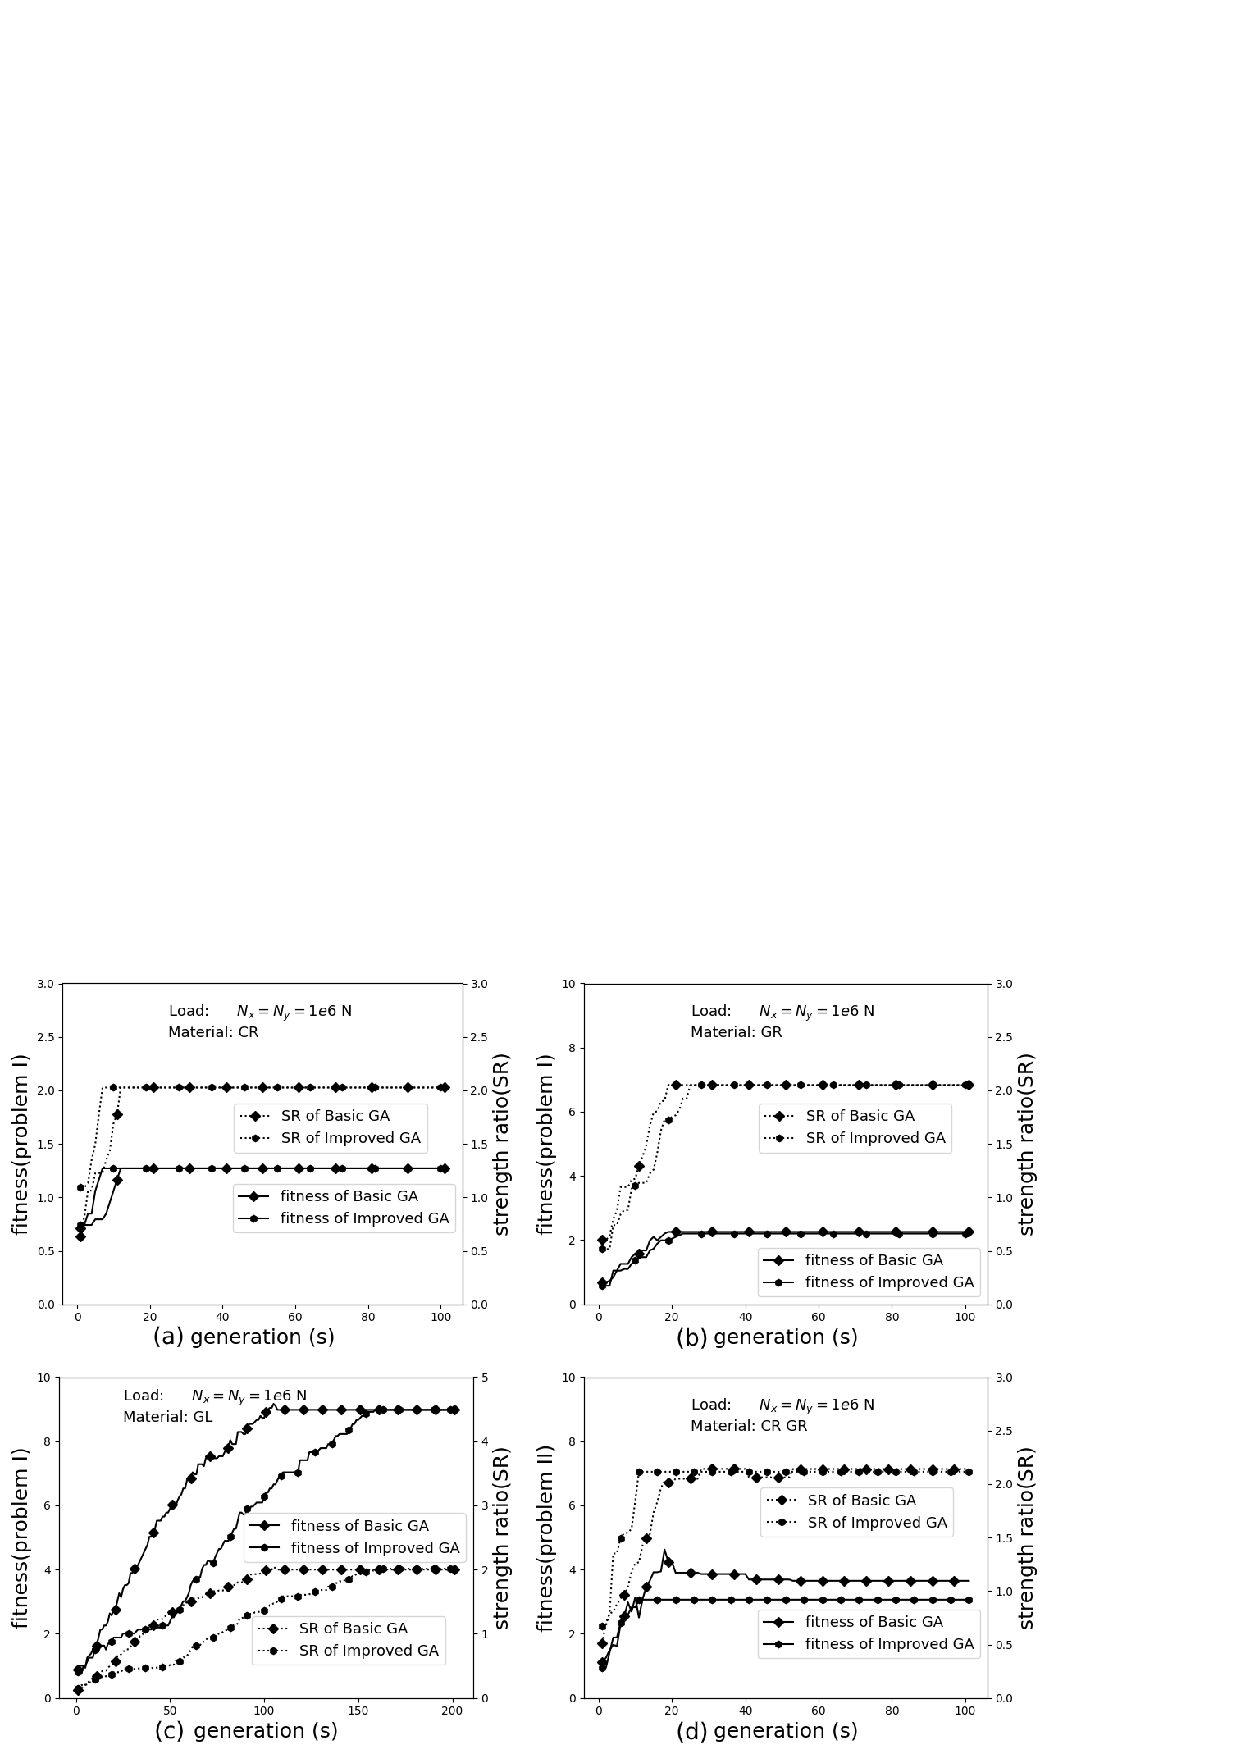
\includegraphics[width=\linewidth]{A_laminate_design_images/NxNy.png}
  \captionof{figure}{GA process under load  $N_x=N_y$ = 1e6 N}
  \label{fig:NxNy}
\end{figure*}


\begin{table*}
\small\sf\centering
\caption{Optimization results}
\begin{tabular}{cccccccc}
	\toprule
	Load(N)                                                 &  Problem  &   Algorithm      & Stacking sequence                                    & Strength ratio  & Mass  &  Cost   & Layer    \\ 
	\midrule																								  
	\multirow{8}{*}{\makecell{$N_x=1e6$ \\ $N_y=1e6$ }}     &       I   &  GA   &  $[\text{-}45_{6}^{cr}/\text{+}45_{6}^{cr}]_s$                        & 2.026           & 1.271 &  192.0  & 24  \\
	                                                        &       I   &  IGA   &  $[\text{-}45_{6}^{cr}/\text{+}45_{6}^{cr}]_s$                        & 2.026           & 1.271 &  192.0  & 24  \\
															&       I   &  GA    &  $[0_6^{gr}/\text{-}45_{4}^{gr}/\text{+}45_{4}^{gr}/90_{7}^{gr}/\bar{90}^{gr}]_s$     & 2.051           & 2.256 &  107.5  & 43  \\
															&       I   &  IGA    &  $[\text{+}45_{10}^{gr}/\text{-}45_{10}^{gr}/\bar{\text{-}45}^{gr}]_s$    & 2.024           & 2.151 &  102.5  & 41  \\
															&       I   &  GA    &  $[\text{-}45_{35}^{gl}/\text{+}45_{36}^{gl}/\bar{\text{+}45}^{gl}]_s$    & 2.001           & 8.980 &  143.0  & 143  \\
															&       I   &  IGA    &  $[\text{-}45_{35}^{gl}/\text{+}45_{36}^{gl}/\bar{\text{+}45}^{gl}]_s$    & 2.001           & 8.980 &  143.0  & 143  \\
															&       II  &  GA    &
	$[\text{-}45_{12}^{gr}/\text{+}45_{5}^{cr}/\text{+}45_{7}^{gr}]_s$         & 2.141
										  & 2.523 & 175& 48  \\
															&       II  &  IGA    &
	$[\text{-}45_{9}^{gr}/\text{+}45_{9}^{gr}/\text{-}45_{2}^{cr}/\text{+}45_{2}^{cr}]_s$         & 2.054
										  & 2.313 & 154& 44  \\
	\bottomrule
\end{tabular}
\label{tab:NxNy}
\end{table*}

\begin{tablenotes}\footnotesize
\item{Subscript "cr" denotes a carbon/epoxy ply, "gr" denotes graphite/epoxy ply, "gl" denotes a
	glass/epoxy ply}
\end{tablenotes}


The GA process can be divided into two phases by whether there are individuals which are appropriate
or not. During the initial phase, no individual's strength ratio is over the specified threshold, so
individuals with bigger fitness are more likely to be chosen as parents, that's why the strength
ratio curves go all the way up to the specified threshold during the first stage; After the initial
phase, the GA produces a bunch of appropriate individuals, and then the target function comes to
play, as you can see from Fig.\ref{fig:NxNy}, the fitness curves are trending to go down, but the
strength ratio curves are keep to greater the specified threshold.


In the first experiment, the applied stress are $N_x=N_y=1e6$ N.  As shown in the
Figure\ref{fig:NxNy}, the Figure \ref{fig:NxNy}(a), (b), and (c) were the experiment results for single material,
Figure \ref{fig:NxNy}(d) is for hybrid composite material. For the single materials, both of the basic GA and improved
GA method obtained the optimal value, but the improved GA converged more slowly than the basic GA.
As it can be seen from Table \ref{tab:NxNy}, a $[\text{-}45_{6}/\text{+}45_{6}]_s$ carbon/epoxy
laminate has the least weight, denoted by $W_{min}$, and a
$[\text{-}45_{35}/\text{+}45_{73}/\text{+}45_{35}]$ graphite/epoxy laminate has the lowest cost,
denoted by $C_{min}$. The $W_{min}$ and $C_{min}$ were used to evaluate the fitness of the second
problem, which is the layup design of hybrid composite material , as shown in sub-figure d,the
improved GA obtained a more appropriate system layup, whose strenght ratio is greater than the
specified safety factor, and weight and cost is less than the result obtained by basic GA method, as
shown in Table \ref{tab:NxNy}. Compared with basic GA, the improved GA method showed more powerful
global search ability in the initial phase.

\begin{figure*}
  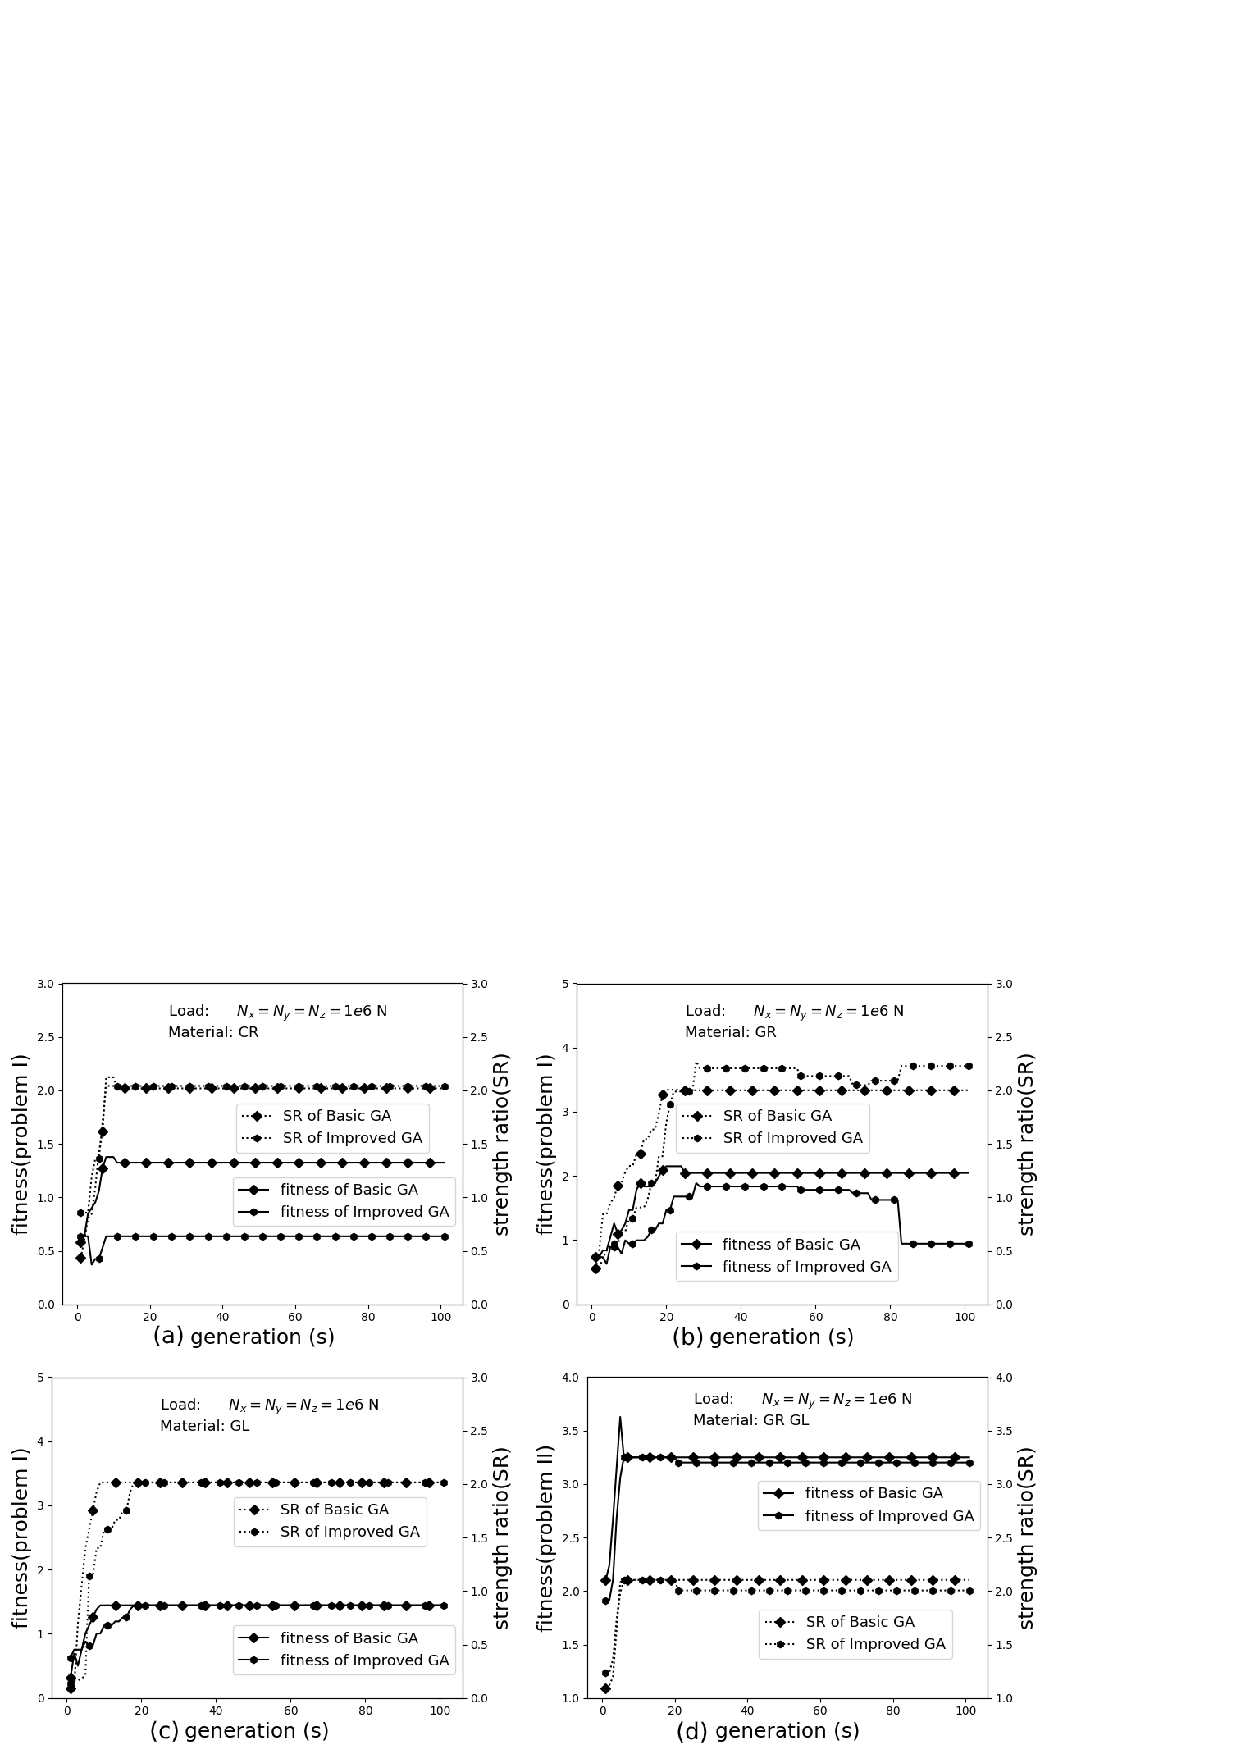
\includegraphics[width=\linewidth]{A_laminate_design_images/NxNyNz.png}
  \captionof{figure}{GA process under load  $N_x=N_y=N_z$ = 1e6 N}
  \label{fig:NxNyNz}
\end{figure*}


\begin{table*}
	\small\sf\centering
	\caption{Optimization results} 
	\begin{tabular}{cccccccc}
	\toprule
	Load(N)                                                 &  Problem  &   Algorithm      & Stacking sequence                                    & Strength ratio  & Mass  &  Cost   & Layer    \\ 
	\midrule																								  
	\multirow{8}{*}{\makecell{$N_{x}=1e6$  \\ $N_{y}=1e6$   \\ $N_{xy}=1e6$ } }  &  I  & GA   &  $[\text{+}45_{11}^{cr}/\text{-}45^{cr}/\bar{\text{+}45}^{cr}]_s$                            & 2.018           & 1.324 &  200.0  & 25  \\
	                                                                             &  I  & IGA  &  $[\text{+}45_{6}^{cr}]_s$                            & 2.041           & 0.636 &  96.0  & 12  \\

																				 &  I  & GA   &  $[0_4^{gr}/\text{+}45_{12}^{gr}/90_3^{gr}/\bar{\text{+}45}]_s$                            & 2.001           & 2.046 &  97.5  & 39  \\
																				 &  I  & IGA  &  $[\text{+}45_{9}^{gr}]_s$                            & 2.227           & 0.945 &  45.0  & 18  \\
																				 &  I  & GA   &  $[\text{+}45_{11}^{gl}/\bar{\text{+}45}^{gl}]_s$                            & 2.015           & 1.444 &  23.0  & 23  \\
																				 &  I  & IGA  &   $[\text{+}45_{11}^{gl}/\bar{\text{+}45}^{gl}]_s$                           & 2.015           & 1.444 &  23.0  & 23  \\
																				 &  II &  GA  &  $[\text{+}45^{gl}/\text{+}45_{8}^{gr}]_s$          & 2.031           & 0.965 &  42.0  & 18 \\
																				 &  II & IGA  &  $[\text{+}45_8^{gr}/\bar{\text{+}45}^{gl}]_s$          & 2.005           & 0.902 &  41.0  & 17 \\
	\bottomrule
\end{tabular}
\label{tab:NxNyNz}
\end{table*}

\begin{comment}
\begin{tablenotes}\footnotesize
     Subscript "cr" denotes a carbon/epoxy ply, "gr" denotes graphite/epoxy ply, "gl" denotes a
	glass/epoxy ply
\end{tablenotes}
\end{comment}

In the second case, the applied stress were $N_x=N_y=N_z=1e6$ N, the experiment results were as
shown in the Figure \ref{fig:NxNyNz}. In the first experiment, as can be seen from Figure \ref{fig:NxNyNz}(a), the improved GA got a
better system layup then result obtained by basic GA; In the second experiment, as shown in the Figure\ref{fig:NxNyNz}(b), during
the initial phase, the fitness curves of basic GA and improved GA went all the way up to the
previous specified threshold, however, the improved GA converged more slowly then the basic GA which
means the search cost of improved GA is greater then basic GA. After the initial phase, the fitness
curve of basic didn't change anymore, it got trapped in local.  However, the fitness curve of
improved GA was gradually going down, at the same time,  the strength ratio curve of improved GA
were keep to be greater then the threshold. It means the improved GA was able to get out of optimum
and obtained a much better system layup.  The improved GA offered more powerful local search
ability. In the third experiment, as shown in Figure \ref{fig:NxNyNz}, both of basic GA and improved
GA obtained the same result, but the improved GA converged more slowly than the basic GA. From these
three experiments for single material, we knew a $[\text{+}45_{6}^{cr}]_s$ carbon/epoxy laminate has
the least mass, and a $[\text{+}45_{11}^{gl}/\bar{\text{+}45}^{gl}]_s$ glass laminate has the least
cost. In the last experiment, the improved GA obtained a little bit better result than the basic GA,
as it shown in Table \ref{tab:NxNyNz}, Compared with the $[\text{+}45_{12}^{cr}]$ laminate, the
weight of a $[\text{+}45_8^{gr}/\bar{\text{+}45}^{gl}]_s$ laminate increases $41.8\%$, however, the
cost decreases $56\%$.

\section{6. Conclusions}
In this paper, a combination of CLT and a variant of GA are employed to minimize the weight and cost
of a single-material and hybrid composite laminate, respectively, under various in-plane loading
cases.  Results are presented in two sections, stacking sequence optimization for a single material
laminate, and weighted  mass and cost optimization of a carbon/epoxy, graphite/epoxy, and
glass/epoxy hybrid laminate.  Furthermore, the performance of the basic GA is improved by changing the
selection strategy.

This variant of GA provides a new approach to deal with constraint search in laminate composite
optimization, and this method is very easy to extend for solving multiple constraints search problem in other
domain. The problem with the current method is to adjust the parameters in the GA to obtain the best
performance. 



\begin{acks}
	This work is supported by
\end{acks}

\bibliographystyle{SageH}
\bibliography{laminate_design}

\end{document}



